\chapter{Evaluierung}\label{evaluierung}

\section{Implementierung} \label{Tests}
Die Implementierung des Min-Conflicts-Embedders und der Automatismus zum Lösen von Bindungs- und Routinganforderungen wurden in der PGAS-Programmiersprache X10 \cite{x10} \cite{pgas} geschrieben. Des Weiteren wurde das vom Lehrstuhl \grqq Hardware-Software-Co-Design\grqq  (Universität Erlangen-Nürnberg) entwickelte CoNoC-Framework in diese parallele, objektorientierte Programmiersprache transformiert und angepasst. Für die Testumgebung wurden zwei Arten von Taskgraphen erstellt und diese mithilfe des Simulators \textit{invadeSIM} \cite{invadeSIM}  ausgewertet.



\section{Testumgebung} \label{Testumgebung1} 
Die Testumgebung besteht aus einem NoC, der jeweils eine Breite und eine Länge von 10 Kacheln besitzt. Die \textit{Unit-} bzw. \textit{LinkAttribute} sind folgendermaßen:
\\
\begin{itemize}
\item \textit{UnitAttribute}
\begin{itemize}
\item \textit{TypeAttribute}\\
Die Hälfte aller Kacheln sind vom Ressourcentyp 0. Der Rest ist Ressourcentyp 1.
\item \textit{UnitWorkloadAttribute}\\
Die Workload einer jeden Kachel beträgt 100.

\end{itemize}
\item \textit{LinkAttribute}
\begin{itemize}
\item \textit{LinkBandwithAttribute}\\
Die maximale Bandbreite eines jeden Links beträgt 10.
\end{itemize}
\end{itemize}

Für die Randbedingungen wurden folgende Vereinfachungen getroffen:
\begin{itemize}
\item \textit{TaskConstraint}
\begin{itemize}
\item \textit{TypeConstraint}\\
Die Hälfte aller Tasks sind vom Ressourcentyp 0. Der Rest ist Ressourcentyp 1.
\item \textit{TaskWorkloadConstraint} \\
Jeder Task benötigt eine Nutzlast von 100.
\end{itemize}
\newpage
\item \textit{CommunicationConstraint}
\begin{itemize}
\item \textit{BandwidthConstraint}\\
Jede Kommunikation benötigt eine Bandbreite von 2.
\item \textit{MaxHopConstraint}\\
Die maximale Distanz zwischen zwei miteinander kommunizierenden Tasks beträgt immer 3.
\end{itemize}
\end{itemize}

Es werden zwei Arten von Taskgraphen näher untersucht. Zum einen ein sequentieller Taskgraph (Abbildung \ref{fig:seq}), bei dem  in einem Zeitabschnitt nur ein Task arbeiten kann, zum anderen ein paralleler Taskgraph (Abbildung \ref{fig:par}), bei dem mehrere Tasks in einem Zeitabschnitt arbeiten können. Für beide Taskgrapharten werden Taskgraphen mit jeweils $n \in \{ 3, 4, 5, 6, 7, 8, 9, 10, 11\}$ Tasks erstellt.
\begin{figure}[H]\centering
  \includegraphics[width = 120mm]{bilder/sequentiell.jpg}
  \caption{Sequentieller Taskgraph mit $n$ Tasks: Ein Kreis repräsentiert einen Task. Ein Rechteck stellt eine Kommunikation dar.
  }\label{fig:seq}
\end{figure}

\begin{figure}[H]\centering
  \includegraphics[width = 70mm]{bilder/parallel.jpg}
  \caption{Paralleler Taskgraph mit $n$ Tasks: Ein Kreis repräsentiert einen Task. Ein Rechteck stellt eine Kommunikation dar.}\label{fig:par}
\end{figure}

\section{Auswertung} \label{Auswertung} 

Abbildung \ref{einbettungszeit} legt dar,  wie viel Zeit der Min-Conflicts-Embedder (Abschnitt \ref{minConflicts} und \ref{minConflictImpl}) benötigt, um sequentielle bzw. parellele Taskgraphen einzuplanen. Die Taskgraphen besitzen die Eigenschaften, die im Abschnitt \ref{Testumgebung1} vorgestellt wurden. Aus der Abbildung \ref{einbettungszeit} ist deutlich zu erkennen, dass beim parallelen Taskgraph  (im Vergleich zum sequentiellen Taskgraph) mit steigender Anzahl der Tasks die benötigte Zeit sich sprunghaft erhöht. So benötigt der Embedder bei einer niedrigen Taskanzahl  für beide Taskgraphtypen etwa die gleiche Zeit, doch etwa ab zehn Tasks divergieren die beiden Graphen. Das Schaubild \ref{mips} stellt den Verlauf der benötigten MIPS (engl. \textit{Million Instructions per Second}) graphisch dar. Aus diesem Diagramm geht hervor, dass der parallele Taskgraph mehr Instruktionen pro Sekunde als der Sequentielle benötigt. Die Graphik \ref{instruktionen} veranschaulicht die Entwicklung der Gesamtzahl der Instruktionen (Formel \ref{formelInstruktionen}).

\begin{equation}
Gesamtzahl der Instruktionen = MIPS * Zeit in Sekunden * 10^6
\label{formelInstruktionen}
\end{equation}

Die Schaubilder verdeutlichen, dass es sinnvoll ist, parallel einzubetten, da man bei parallelen Taskgraphen (siehe Abbildung \ref{fig:par}) für die Tasks $t_2$ bis $t_{n-1}$ simultan eine Lösung finden kann. Somit kann die benötigte Zeit verkürzt werden. Das Programm wurde mit der Sprache  X10 \cite{x10}  programmiert. Dies ist eine parallele, objektorientierte Programmiersprache, die speziell für high-end Hardware mit bis zu 10.000 Hardware-Threads \cite{x10Spezi} , entwickelt wurde. So sollten die  kommenden Aufgaben für dieses Projekt sein, einen parallel agierende Embedder zu implementieren, der auf Basis eines Backtracking-Ansatzes \cite{jaeger} arbeitet.
\begin{figure}
\centering
        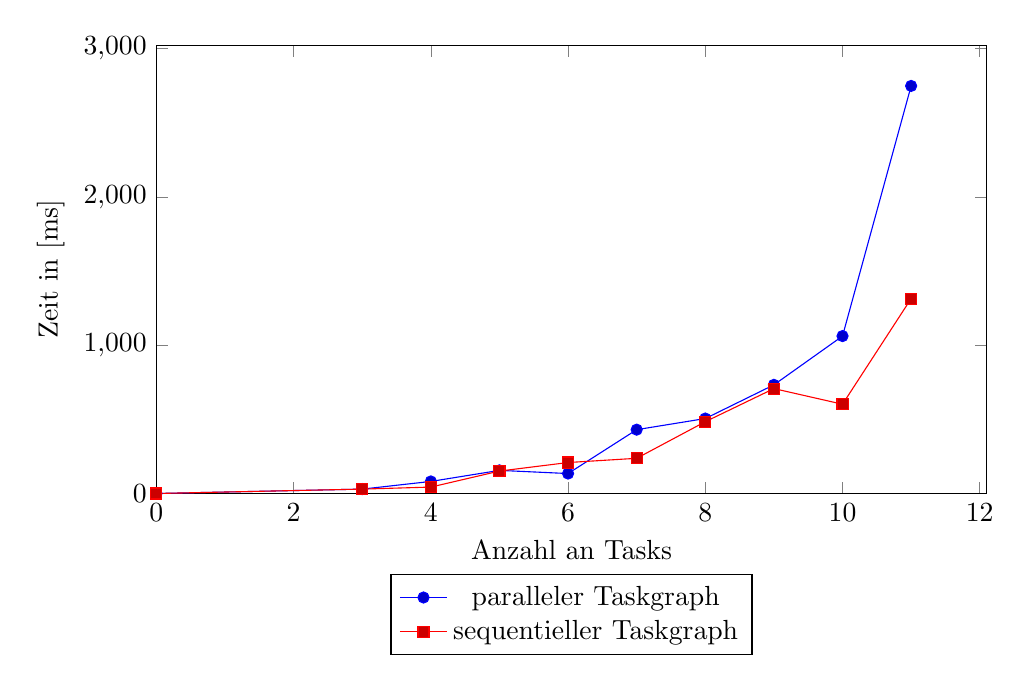
\begin{tikzpicture}
         \pgfplotsset{every axis legend/.append style={at={(0.5,-0.18)}, anchor=north}}
                \begin{axis}[xmin=0,ymin=0,
                xlabel={Anzahl an Tasks},
                ylabel={Zeit in [ms]},
                width=1.0\textwidth,
      height=0.6\textwidth]
          %      \addplot [domain=0:80, samples=60]{1750.763223011357};
                        \addplot coordinates {
                        (0, 0)
                        (3, 29.628)
                        (4, 81.35)
                        (5, 155.8845)
                        (6, 134.531)
                        (7, 430.3)
                        (8, 505.35)
                        (9, 732.4)
                        (10, 1061.243)
                       (11, 2747.662)
};

                        \addplot coordinates {
                        (0, 0)
                         (3, 29.628)
                         (4, 43.2675)
                        (5, 151.2)
                        (6, 208.794)
                        (7, 237.3)
                        (8, 483.9455)
                        (9, 707.2)
                        (10, 601.821)
                       (11, 1313.9)
};

         \legend{paralleler Taskgraph, sequentieller Taskgraph}
                \end{axis}
        \end{tikzpicture}
\caption{Zeit, die der Embedder für die Einplanung benötigt.}
\label{einbettungszeit}
\end{figure}  





\begin{figure}
\centering
        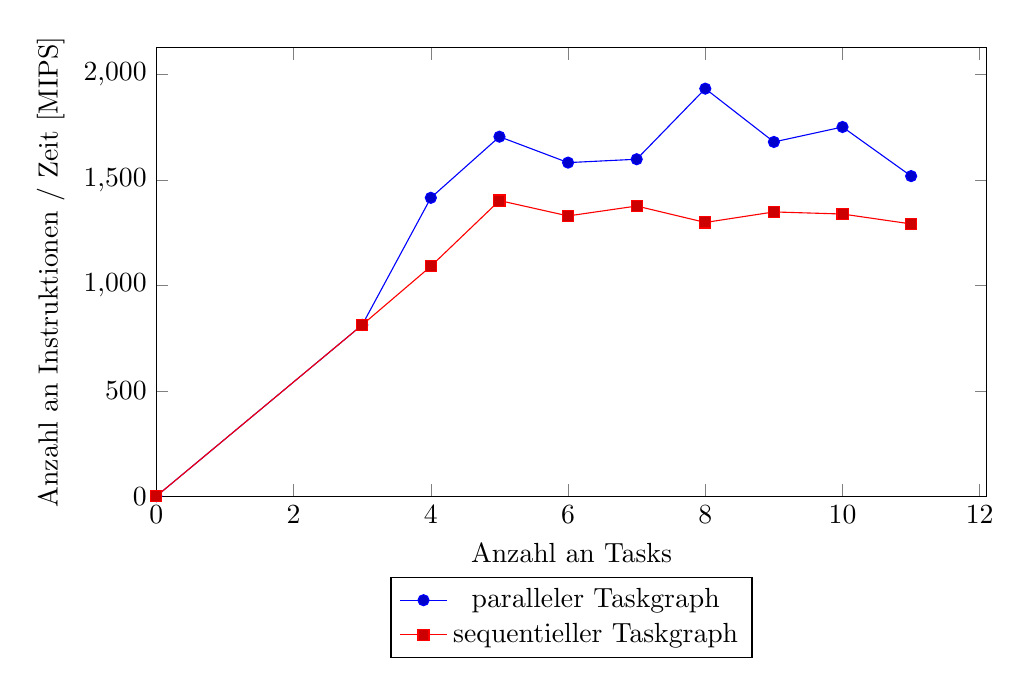
\begin{tikzpicture}
         \pgfplotsset{every axis legend/.append style={at={(0.5,-0.18)}, anchor=north}}
                \begin{axis}[xmin=0,ymin=0,
                xlabel={Anzahl an Tasks},
                ylabel={Anzahl an Instruktionen / Zeit [MIPS]},
                width=1.0\textwidth,
      height=0.6\textwidth]
%                \addplot [domain=0:80, samples=60]{1750.763223011357};
                        \addplot coordinates {
                        (0, 0)
                        (3, 813)
                        (4, 1416)
                        (5, 1706)
                        (6, 1583)
                        (7, 1599)
                        (8, 1934)
                        (9, 1681)
                        (10, 1752)
                       (11, 1519)
};

                        \addplot coordinates {
                        (0, 0)
                         (3, 813)
                         (4, 1091)
                        (5, 1403)
                        (6, 1330)
                        (7, 1377)
                        (8, 1299)
                        (9, 1349)
                        (10, 1339)
                       (11, 1292)
};

        \legend{paralleler Taskgraph, sequentieller Taskgraph}
                \end{axis}
        \end{tikzpicture}
\caption{Anzahl der MIPS, die der Embedder benötigt.}
\label{mips}
\end{figure}  

\begin{figure}
\centering
        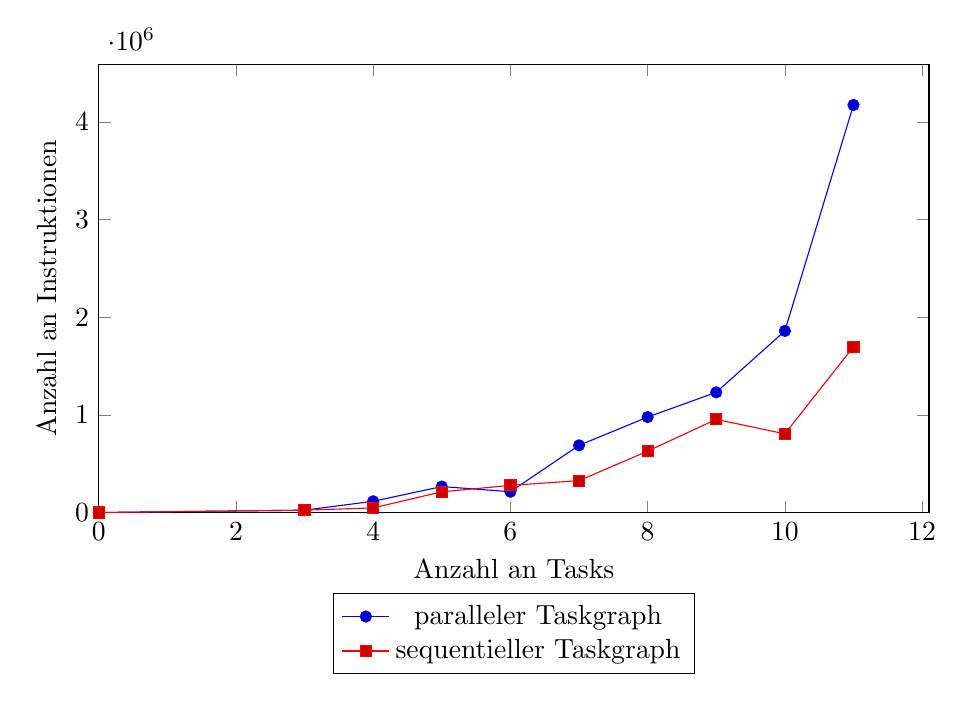
\begin{tikzpicture}
         \pgfplotsset{every axis legend/.append style={at={(0.5,-0.18)}, anchor=north}}
                \begin{axis}[xmin=0,ymin=0,
                xlabel={Anzahl an Tasks},
                ylabel={Anzahl an Instruktionen },
                width=1.0\textwidth,
      height=0.6\textwidth]
%                \addplot [domain=0:80, samples=60]{1750.763223011357};
                        \addplot coordinates {
                        (0, 0)
                        (3,24088)
(4,115192)
(5,265939)
(6,212963)
(7,688050)
(8,977347)
(9,1231164)
(10,1859298)
(11,4173699)


};

                        \addplot coordinates {
                        (0, 0)
                         (3,24088)
(4,47205)
(5,212134)
(6,277696)
(7,326762)
(8,628645)
(9,954013)
(10,805838)
(11,1697559)

};

        \legend{paralleler Taskgraph, sequentieller Taskgraph}
                \end{axis}
        \end{tikzpicture}
\caption{Gesamtzahl der Instruktionen, die der Embedder benötigt.}
\label{instruktionen}
\end{figure}  
